%%=============================================================================
%% Methodologie
%%=============================================================================

\chapter{\IfLanguageName{dutch}{Methodologie}{Methodology}}%
\label{ch:methodologie}

%% TODO: Hoe ben je te werk gegaan? Verdeel je onderzoek in grote fasen, en
%% licht in elke fase toe welke stappen je gevolgd hebt. Verantwoord waarom je
%% op deze manier te werk gegaan bent. Je moet kunnen aantonen dat je de best
%% mogelijke manier toegepast hebt om een antwoord te vinden op de
%% onderzoeksvraag.

Zoals eerder vermeld zal, dit onderzoek zich focussen op het voorstel dat Bluetooth Low Energy een optimale oplossing is voor asset tracking in de bouwindustrie. Tegenwoordig worden daar vooral andere technologieën voor gebruikt. BLE zit daar reeds tussen, maar in veel mindere mate. In dit gedeelte van de scripte zal er een requirements-analyse uitgevoerd worden waarin alle functionele en niet-functionele vereisten uitgezocht zullen worden. Vervolgens zal er een long en short list opgesteld worden waarin alle technologieën, die vandaag de dag voornamelijk gebruikt worden, aan bod zullen komen, vergeleken en gefilterd zullen worden op geschiktheid. Hierin zal ook een grondige beschrijving aanwezig zijn van alle voor -en nadelen van BLE. Ook bestaat dit deel uit een toelichting van alle geschikte protocols, software en hardware. Op basis hiervan zal er een experimenteel onderzoek plaatsvinden aan de hand van een zelfontwikkelde Android-applicatie.

\subsection{Requirements-analyse}
Om een correcte vergelijking te maken tussen de meest frequent voorkomende technologieën die gebruikt worden om zaken als machines, voertuigen, werkmateriaal of personeel te traceren op een bouwwerf moet er enkele functionele en niet-functionele vereisten opgelijst worden. Deze zullen de beslissingsfactoren zijn waarom een bepaalde technologie boven een ander wordt verkozen. Aan de hand van deze factoren zal de hierna opgelijste long list geoptimaliseerd worden naar een short list waarin enkel de beste kandidaten nog aanwezig zijn.\\

Voor functionele vereisten gaan we kijken naar zaken die definiëren wat het systeem moet doen om aan de behoeften en verwachtingen van de gebruiker te voldoen. Zaken die hier onder ressorteren zijn bijvoorbeeld het kunnen traceren van een bepaald activa binnen een bepaalde voorafbepaalde radius en een liefst zo klein mogelijke foutmarge hebben tussen de locatie in werkelijkheid en degene aangegeven op de gebruikte software. Dit laatste, ook wel traceernauwkeurigheid genoemd, is een interessant gegeven om te vergelijken aangezien bepaalde technologieën bekend staan om een accuratere plaatsbepaling te hebben dan andere.\\

Voor niet-functionele vereisten gaan we kijken naar zaken die de werking van een systeem kunnen beoordelen, in plaats van specifiek gedrag. Deze eisen staan tegenover de functionele eisen, die hierboven beschreven staan, die specifiek gedrag of functies definiëren. Vereisten die hier ressorteren zijn zaken als initiële en operationele kosten, beveiliging, installatiegemak en het onderhoud van hardware.

\subsection{Long list}
De meest frequent voorkomende technologieën om activa te traceren op een bouwwerf zijn in de literatuurstudie van deze scriptie reeds opgelijst en beschreven geweest. In dit gedeelte van de scriptie zullen deze technologieën met elkaar vergeleken worden aan de hand van functionele en niet-functionele vereisten die in de rubriek hierboven vastgesteld zijn geweest.\\

De zes reeds beschreven technologieën zijn Global Positioning System (GPS), Radio Frequentie Identifier(RFID), Ultra-wideband (UWB), Barcode, QR Codes en Bluetooth Low Energy (BLE). Deze technologieën zullen met elkaar vergeleken worden door middel van volgende functionele en niet-functionele criteria:

\begin{itemize}
    \item Dekking
    \item Traceernauwkeurigheid
    \item Kosten
    \item Beveiliging
    \item Installatiegemak
    \item Onderhoud
\end{itemize}

Uit deze vergelijking zal een kleinere lijst gevormd worden (short list) met de technologieën die het meest potentieel hebben. Deze zullen dan meer in detail bekeken en vergeleken worden welke van de vijf technologieën het meest geschikt is voor de use-case die deze scriptie behandeld namelijk asset tracking op een bouwwerf. Hieruit zal een tijdelijke conclusie opgebouwd worden.\\

\begin{table}
\tiny
\begin{tabularx}{\textwidth} { 
        | >{\raggedright\arraybackslash}X 
        | >{\centering\arraybackslash}X 
        | >{\centering\arraybackslash}X 
        | >{\centering\arraybackslash}X 
        | >{\centering\arraybackslash}X 
        | >{\centering\arraybackslash}X 
        | >{\centering\arraybackslash}X 
        | >{\centering\arraybackslash}X | }
\hline
 & GPS & RFID & UWB & Barcode & QR Codes & BLE \\
\hline
Werkgebied & $\infty$ & <100m & <200m & Nvt & Nvt & < 100m\\
Nauwkeurigheid & <10m & <10cm & <30cm & Nvt & Nvt & 2-3m \\
Beveiliging & \\
Installatiekosten & Goedkoop & Duur & Goedkoop & Goedkoop & Goedkoop & Goedkoop \\
Onderhoudskosten & Duur & Goedkoop & Goedkoop & Goedkoop & Goedkoop & Goedkoop  \\
Tag prijs & \euro25 tot \euro50 & 50 cent tot \euro100 & >\euro100 & Afhankelijk & Gratis - afhankelijk & \euro5 tot \euro100 \\
Functie & Identificatie en lokalisatie & Identificatie & Identificatie en lokalisatie & Identificatie & Identificatie & Identificatie en lokalisatie \\
\hline
\end{tabularx}
\caption{Een vergelijking van alle mogelijke asset tracking technologieën volgens bepaalde criteria. De meeste data voor deze tabel werd uit een eerder uitgevoerde studie overgenomen, geschreven door \textcite{Ahmed2020}.}
\label{tab:technologies}
\end{table}

Uit tabel \ref{tab:technologies} kunnen verschillende dingen gelezen en afgeleid worden. Uit deze oppervlakkige verschillen kan al snel een conclusie gemaakt worden welke technologieën meer geschikt zijn dan anderen, hieruit ontstaat dan een specifiekere lijst met kandidaten volgens geschiktheid. \\

Het eerste criteria is werkgebied. Dit toont de afstand waarop een tag bereikt kan worden. Als gekeken wordt naar de verschillende technologieën zijn er meteen zaken die opvallen. Beginnend bij GPS waarbij kan geobserveerd worden dat het werkbereik oneindig is. Dit betekend dat een GPS tag van overal ter wereld bereikt kan worden. Dit is logisch aangezien een GPS tag een simkaart bevat die de positionele en soms ook andere data doorstuurt naar de servers van de gekozen provider over het mobiel netwerk, zoals reeds uitgelegd is geweest. Wat voor dit criteria nog opvalt is dat er bij barcode en QR code 'niet van toepassing' bijstaat. Vanzelfsprekend aangezien barcode en QR code functioneel niet geschikt zijn voor lokalisatie. Barcodes en QR codes kunnen wel van op een afstand gescand worden, maar dit is enkel mogelijk indien er een directe gezichtslijn is met de barcode of QR code. De afstand wordt uiteindelijk bepaald door de resolutie van de barcode of QR code. Als gekeken wordt naar de overige technologieën kan geobserveerd worden dat RFID en BLE gelijk staan en dat UWB het grootste werkgebied heeft. Deze waarden zijn zeker niet vast en kunnen veel afwijken. Dit is data verzameld door \textcite{Roberts2006} en wijkt voor RFID soms honderden meters af van andere data op het internet. Het werkgebied van technologieën als RFID, UWB of BLE hangt dus volledig af van het soort tag. 

RFID heeft twee soorten tags, namelijk actief en passieve tags. Actieve tags hebben een externe energiebron, meestal een batterij. Dit betekent dat actieve tags van veel verder gelezen kunnen worden. Passieve tags halen hun vermogen uit de transmissie van de lezer via inductieve koppeling \autocite{Roberts2006}. De passieve tags reageren dan op dat signaal. Inductieve koppeling vereist gewoonlijk dat het signaal van redelijk dichtbij verstuurd wordt. Actieve tags langs de andere kant communiceren gewoonlijk via propagatiekoppeling en reageren op de transmissie van de lezer door gebruik te maken van intern vermogen, zoals eerder vermeld.

Net zoals bij RFID is het werkgebied van UWB en BLE tags volledig afhankelijk van het soort tag dat gebruikt wordt. In het geval van BLE en UWB wordt het werkbereik bepaald door de combinatie van chipset, antenne en pad verlies. Pad verlies is de maat waarin vermogen van een radiosignaal uitgedrukt wordt dat verloren gaat onderweg van de zender tot de ontvanger \autocite{Tosi2017}. Het wordt gedefinieerd als het verschil tussen het vermogen van de zender en de gevoeligheid van de ontvanger, beiden uitgedrukt in dBm (decibel-milliwatts). Het verband tussen pad verlies en afstand (d) wordt in figuur \ref{fig:range} weergegeven. De vergelijking is wel alleen maar geldig voor een isotrope antenne en houdt geen rekening met eventuele verliezen, reflectie, ruis of obstakels in de omgeving. Het werkgebied kan door deze factoren drastisch variëren. Dit geld natuurlijk voor alle technologieën waar radio frequentie aan te pas komt.\\ 

\begin{figure}
    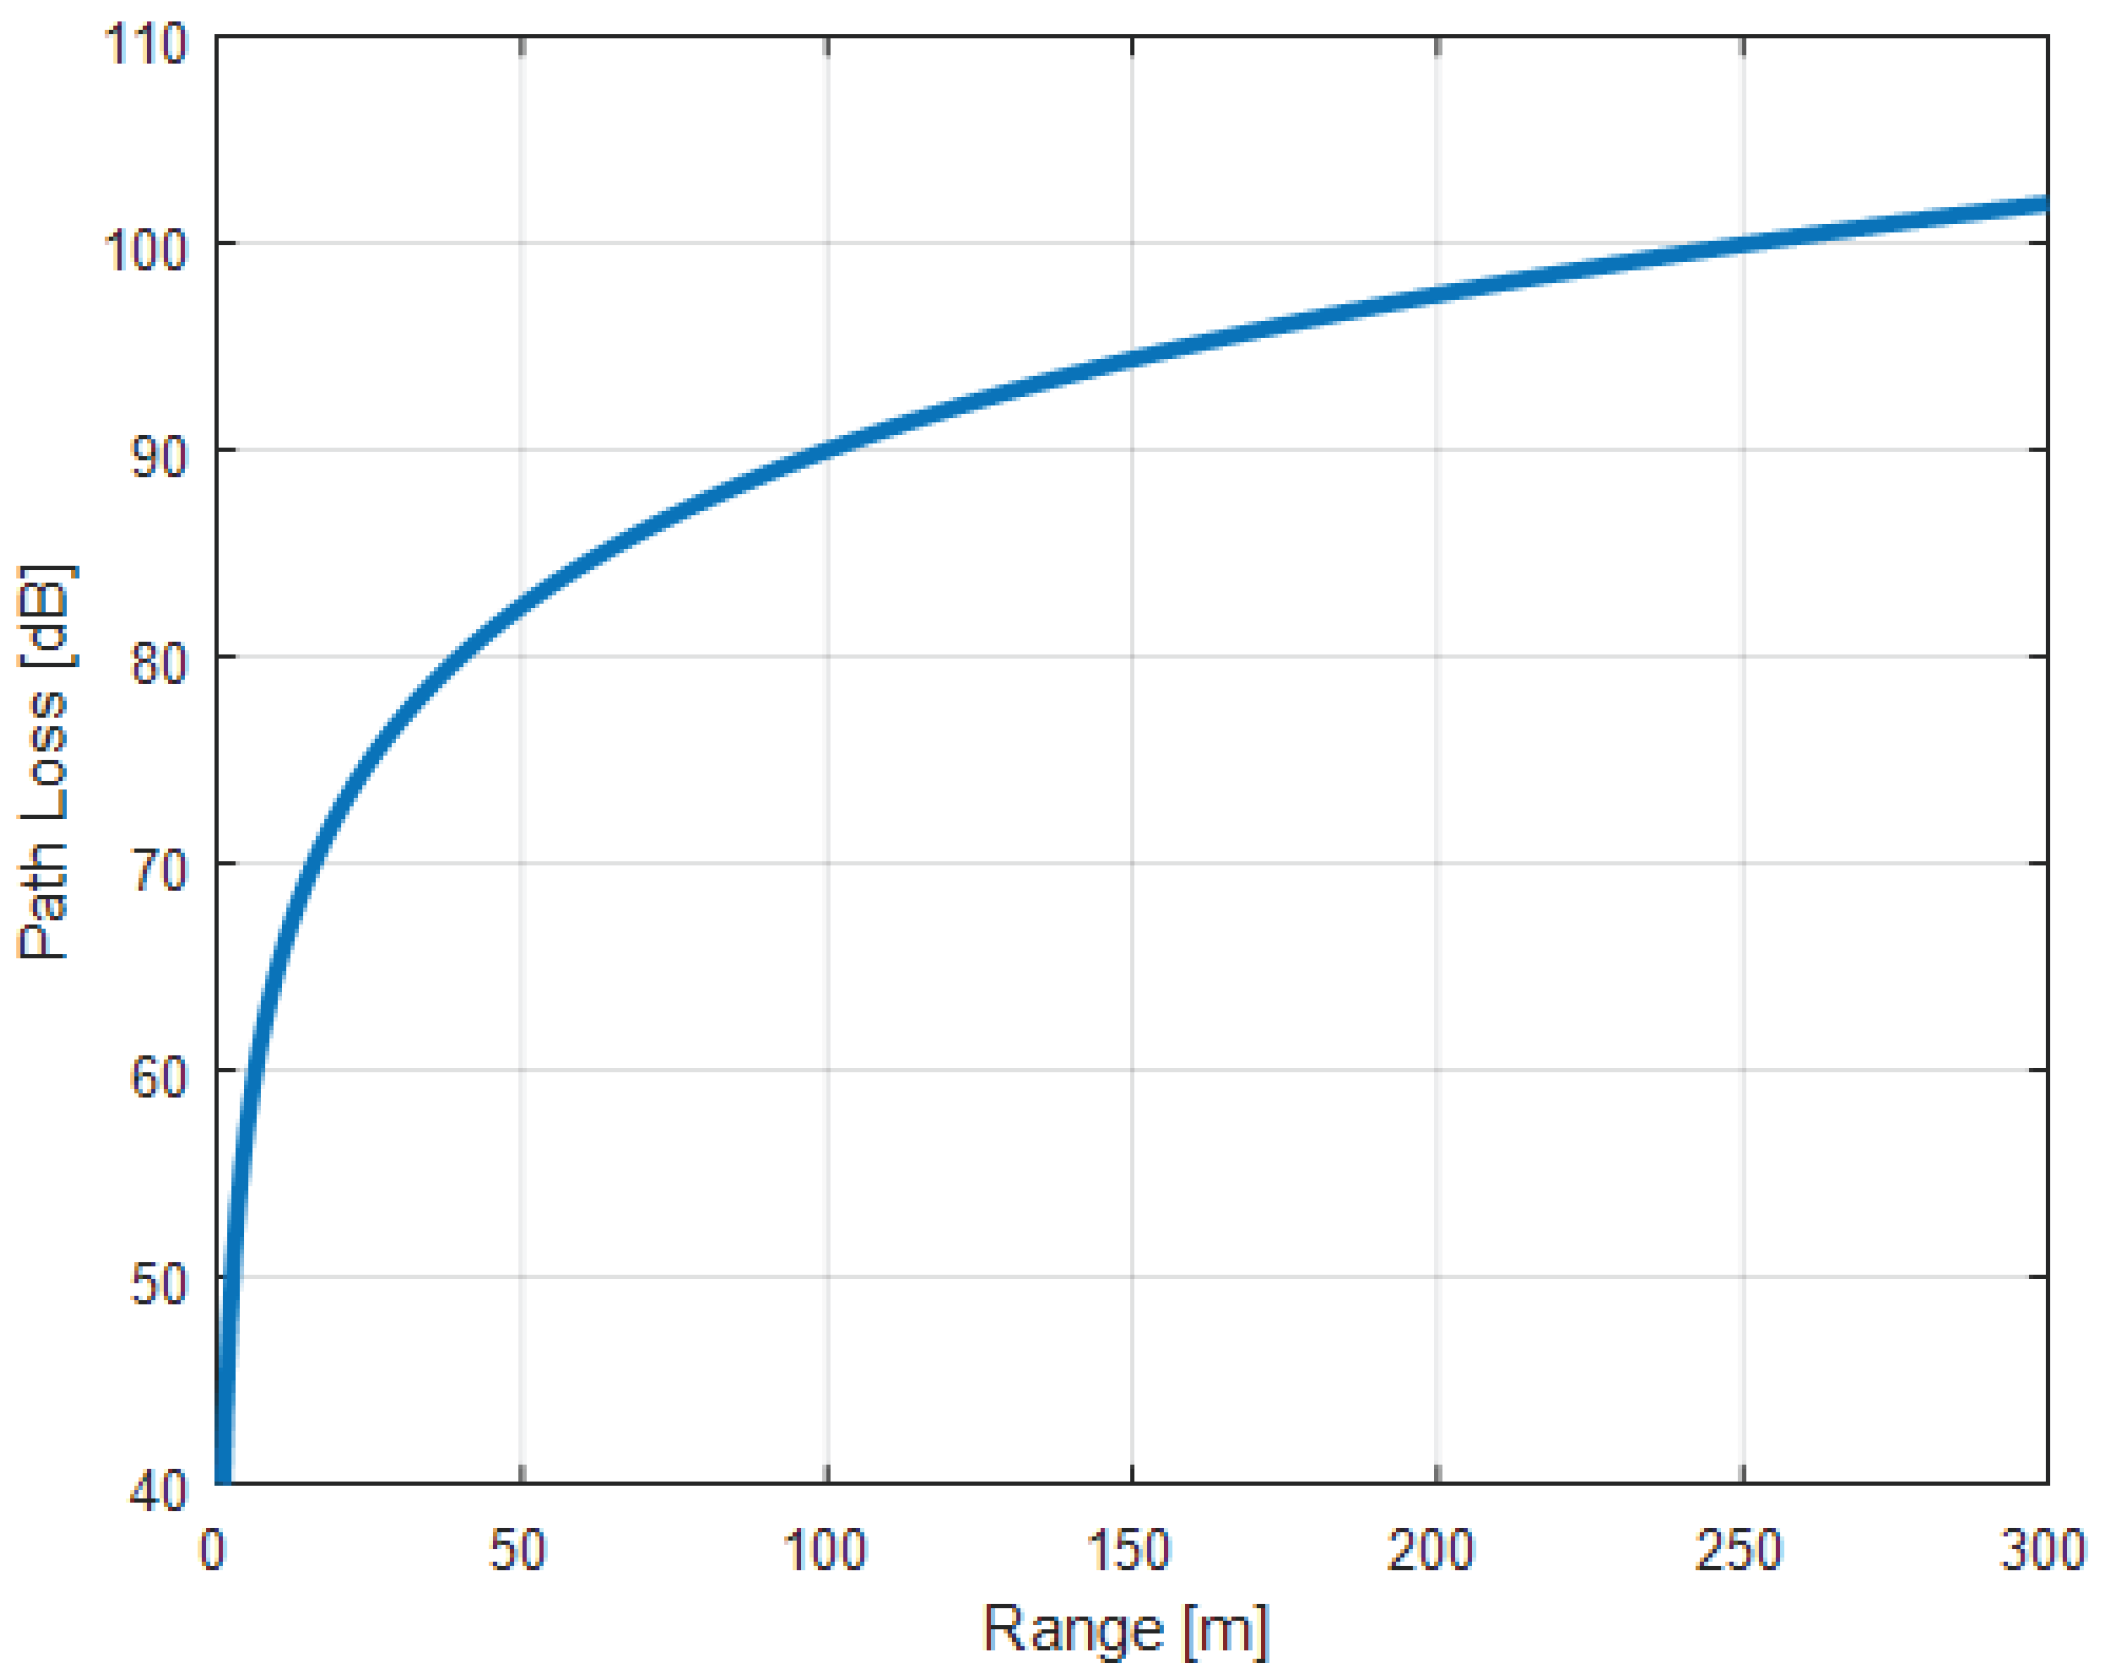
\includegraphics[\textwidth]{range.png}
    \caption[Barcode]{Een grafische representatie van pad verlies, verkregen door vergelijking \ref{pathloss} uit \autocite{Tosi2017}}
    \label{fig:range}
\end{figure}

\begin{equation}
    \label{pathloss}
    pathloss=40+25×log(d)
\end{equation}
\\

Onderhoudskosten - beter dan dit kan natuurlijk niet, maar dit komt met een prijskaartje

De laatste criteria is de functie van de technologieën. Aan de hand van dit criteria kan makkelijk bepaald worden wat de mogelijkheden zijn van een bepaalde technologie. Iedere technologie blijkt de mogelijkheid tot identificatie te hebben maar wat voor dit vergelijkend onderzoek belangrijk is, is of de technologie mogelijkheid biedt tot lokalisatie. Als we de technologieën overlopen zien we meteen twee technologieën die eruit springen. Dit zijn barcode en QR code. Bij deze twee is het niet mogelijk om op een of andere manier de locatie van het activa waaraan de code bevestigd is te lokaliseren. Voor de onderzoeksvraag van deze scriptie is het wel van cruciaal belang dat dit mogelijk is en daarom zullen we deze twee technologieën achterwegen laten voor deze vergelijkende studie.\\

Het tweede criteria is traceernauwkeurigheid. Indien een bouwwerf van kleine oppervlakte is of de te traceren activa dicht bij elkaar staan is het van belang dat deze makkelijk gelokaliseerd kan worden en dat deze activa niet met elkaar verwisseld worden door een slechte traceernauwkeurigheid. Aangezien barcode en QR code niet van op afstand traceerbaar zijn zullen deze vanzelfsprekend niet meegerekend worden. De traceernauwkeurigheid bij deze twee technologieën zal altijd 100\% zijn aangezien de activa eerst handmatig gelokaliseerd moet worden voor de code gescand kan worden.

De waarden van de andere technologieën zijn vrij verschillend. De technologie die er een beetje uitsteekt is GPS. Dit is geweten dat GPS in het algemeen het minst exact de locatie van iets weergeeft. De afstand kan variëren van een paar meter tot precies. Zo een afwijking kan veroorzaakt worden door verschillende zaken zoals satellietgeometrie, signaal obstructie of atmosferische omstandigheden.

Bij de andere technologieën is er nog maar een technologie dat meer dan een meter afwijkt en dit is BLE. Om de afstand te bepalen tussen een zendende (TX) en een ontvangende (RX) node wordt bij BLE Received Signal Strength Indicator (RSSI) gebruikt. Dit is de reden voor de afwijking bij de traceernauwkeurigheid van BLE. RSSI wordt berekend aan de hand van vergelijking \ref{rssi}.

\begin{equation}
    \label{rssi}
    RSSI=−10×N×log(d)+a
\end{equation}

Hierin is $N$ een constante die als één wordt aangenomen, $d$ de afstand in meters tussen de twee apparaten en $a$ het vermogen van de TX op één meter afstand.

\subsection{Short list}
Twee technologieën zijn duidelijk niet geschikt voor asset tracking op een bouwwerf, namelijk barcode en QR code. De reden hiervoor is dat activa waarop een code bevestigd is niet van op afstand gelokaliseerd kan worden. Dit is van cruciaal belang indien men snel activa wil lokaliseren in een complexe en drukke omgeving als een bouwwerf. Indien de overgebleven technologieën nog eens naast elkaar gelegd worden komen we bij tabel \ref{tab:technologies2} uit. Hier zijn er wat extra criteria bijgevoegd aangezien de technologieën op specifiekere vlakken met elkaar verschillen die in de praktijk minstens even belangrijk zouden kunnen zijn om de meest geschikte technologie voor asset tracking op een bouwwerf te kiezen. Dit zijn zaken zoals de levensduur van batterijen, energieverbruik en of de technologie compatibel is met smartphones. 

\begin{table}
    \tiny
    \begin{tabularx}{\textwidth} { 
            | >{\raggedright\arraybackslash}X 
            | >{\centering\arraybackslash}X 
            | >{\centering\arraybackslash}X 
            | >{\centering\arraybackslash}X 
            | >{\centering\arraybackslash}X 
            | >{\centering\arraybackslash}X 
            | >{\centering\arraybackslash}X 
            | >{\centering\arraybackslash}X | }
        \hline
        & GPS & RFID & UWB & BLE \\
        \hline
        Functie & Identificatie en lokalisatie & Identificatie & Identificatie en lokalisatie & Identificatie en lokalisatie \\
        Werkgebied & $\infty$ & <100m & <200m & < 100m\\
        Nauwkeurigheid & <10m & <10cm & <30cm & 2-3m \\
        Beveiliging & \\
        Installatiekosten & Goedkoop & Duur & Goedkoop & Goedkoop \\
        Onderhoudskosten & Duur & Goedkoop & Goedkoop & Goedkoop  \\
        Tag prijs & \euro25 tot \euro50 & 50 cent tot \euro100 & >\euro100 & \euro5 tot \euro100 \\
        \hline
        Batterij & <3 jaar & 3-5 jaar & <2 jaar & 2-5 jaar \\
        Energieverbruik & Laag & Laag/Hoog & Laag & Laagst\\
        Smartphone compatibiliteit & $\bullet$ & & $\bullet$ & $\bullet$ \\
        \hline
    \end{tabularx}
    \caption{Een nauwkeurigere vergelijking van verschillende geschikte asset tracking technologieën volgens bepaalde criteria. De data voor deze tabel werd net zoals bij tabel \ref{tab:technologies} uit een eerder uitgevoerde studie overgenomen, geschreven door \textcite{Ahmed2020}.}
    \label{tab:technologies2}
\end{table}

smartphone compatibliteit rfid https://gadgetfaculty.com/smartphone-rfid-reader-rfid-tag/
uhf is not compatible with nfc

\subsection{Conclusie vergelijkende studie}
Hier zal een conclusie opgesteld worden aan de hand van de vergelijkende studie die uitgevoerd is geweest in de rubriek hierboven. Deze conclusie, samen met de uitkomst van de proof of concept zullen dan de eindconclusie bepalen.

%TODO:Vergelijking tussen de verschillende techologien, tabel maken en alles volluit uitgeschreven uitgelegd erbij

%TODO: De eerste fase is een introductie over de pro-blematiek. Dit wordt gerealiseerd door een gron-dige studie van vakliteratuur, zoals wetenschap-pelijke teksten of blogs. Hieruit volgt een tekstdie alle vereisten aanhaalt voor een optimale op-lossing. De geschatte duurtijd van deze fase be-draagt twee weken.
\subsection{Voordelen van BLE asset tracking}
Hier zullen alle voordelen van BLE asset tracking beschreven worden en nog een vergeleken worden met andere technologieën.
%TODO: De tweede fase houdt een analyse in van wetenschappelijke teksten, met als resultaat een uitgebreide tekst over de voordelen van BLE asset tracking, ten opzichte van technologieën die van-daag de dag gebruikt worden. Hiervoor is een week genoeg.
\subsection{Nadelen van BLE asset tracking}
Hier zullen alle nadelen van BLE asset tracking beschreven worden en nog een vergeleken worden met andere technologieën.
%TODO: De derde fase is opnieuw een beschrijving,maar dan over de valkuilen van BLE asset tracking.  Deze fase van het onderzoek brengt alle mogelijke tekortkomingen in kaart.  Ook voor deze fase is een week voldoende.
\subsection{Toelichting van protocols, hardware en software}
In dit gedeelte zal een toelichting van alle bestaande protocols van beacons en tags beschreven worden. Hierbij wordt er gezocht naar de meest geschikte hardware waarbij er nauwkeurig afgewogen moet worden tussen kosten en functionaliteit. 
%TODO: De vierde fase bestaat uit het toelichten van de meest geschikte protocols, compatibiliteit van software en hardware ,zoals beacons en gateways.Hierbij wordt er gezocht naar de meest geschikte hardware waarbij er nauwkeurig afgewogen moet worden tussen kosten en functionaliteit. Vervolgens wordt er een veldonderzoek uitgevoerd om,naargelang de vereisten, de keuze te maken op welke manier de app ontwikkeld zal worden. Tot slot zullen alle beschikbare protocols in kaart gebracht worden. De geschatte duurtijd van deze fase bedraagt drie weken.
\subsection{Proof of Concept}

